% =====================================================================
% THIS FILE IS THE SOURCE. Edit it, then rebuild the PDF with:
%     bash tools/compile.sh Unit_10_Estimation_and_the_Bootstrap
% (run from the Course_Rewrite folder; it compiles twice and reports
%  page count, overfull boxes, and em dashes)
%
% Do not edit the PDF directly. Figures are the fig_*.pdf files in this
% folder, regenerated by tools/make_module*_slide_figs.py.
%
% Originally converted from the 15-module draft by a one-shot script now
% parked in tools/one_shot_generators/. Re-running those would discard
% anything you change here, so they are kept out of tools/ on purpose.
% =====================================================================
\documentclass[aspectratio=169]{beamer}
\usetheme{default}
\usefonttheme{professionalfonts}
\usepackage{amsmath, amssymb, amsfonts}
\usepackage{graphicx}
\usepackage{booktabs}
\usepackage{bm}
\usepackage{hyperref}

\mode<presentation> {
    \usetheme{Frankfurt}
    \usecolortheme{default}
}

\newcommand{\xbar}{\bar{x}}
\newcommand{\yhat}{\hat{y}}
\newcommand{\E}[1]{E[#1]}
\newcommand{\SD}[1]{\mathrm{SD}(#1)}

\newenvironment{principle}[1]{\begin{block}{\textbf{Principle:} #1}}{\end{block}}
\newenvironment{trap}[1]{\begin{alertblock}{\textbf{Trap:} #1}}{\end{alertblock}}
\newenvironment{practice}[1]{\begin{exampleblock}{\textbf{In practice:} #1}}{\end{exampleblock}}
\newenvironment{interview}[1]{\begin{exampleblock}{\textbf{You may be asked:} #1}}{\end{exampleblock}}
\newenvironment{yourturn}[1]{%
  \setbeamercolor{block title}{fg=white,bg=orange!80!black}%
  \setbeamercolor{block body}{bg=orange!12}%
  \begin{block}{\textbf{Your turn:} #1}}{\end{block}}
\newenvironment{livedemo}[1]{%
  \setbeamercolor{block title}{fg=white,bg=teal!80!black}%
  \setbeamercolor{block body}{bg=teal!12}%
  \begin{block}{\textbf{Live demo:} #1}}{\end{block}}
\newenvironment{llmcheck}[1]{%
  \setbeamercolor{block title}{fg=white,bg=violet!75!black}%
  \setbeamercolor{block body}{bg=violet!10}%
  \begin{block}{\textbf{LLM check:} #1}}{\end{block}}

\title{Estimation, Likelihood, and the Bootstrap}
\subtitle{Unit 10: Turning a Sample Into a Number You Can Defend}
\author{Stat 220 \textbar{} Statistics for Data Science}
\date{}

\begin{document}

\begin{frame}
  \titlepage
\end{frame}

% ======================================================================
\section{Why}
% ======================================================================
\begin{frame}{Where this fits}
\begin{itemize}
  \item We know what randomness looks like and how averages behave. Now the practical question:
        given data, \textbf{how do you produce the number}, and how do you attach uncertainty to
        it?
  \item Sometimes the quantity is a mean and there is a formula. Usually it is a median, a ratio,
        a 90th percentile, or a model output, and there is not.
  \item This module gives you two general-purpose tools that work when formulas run out:
        \textbf{likelihood} and \textbf{the bootstrap}.
\end{itemize}
\begin{principle}{judge the recipe, not one result}
Judge the recipe, not the number it happened to produce this time. The right question is always
``if I ran this procedure on a fresh sample, how far off would it typically be?''
\end{principle}
\end{frame}

\begin{frame}{Live experiment: the serial-number contest}
\begin{livedemo}{estimate what you cannot see}
I have a bag of tickets numbered $1$ through $N$. You do not know $N$. I draw \textbf{five}
tickets and write the numbers on the board.
\begin{itemize}
  \item In teams of three, write down a \textbf{formula} that turns those five numbers into a
        guess for $N$. Any formula, as long as it is a rule I can apply mechanically.
  \item Then I will run every team's formula on \textbf{50 fresh draws} from the same bag and
        score you by average squared error.
\end{itemize}
\end{livedemo}
\vspace{0.2em}
{\tiny\textit{Materials: a bag of numbered tickets, or just draw them on screen. Time: 15 minutes, including scoring each team's rule on fresh draws.}}
\centering\small The winner is not the team that guessed closest once. It is the team whose
\emph{rule} performs best repeatedly.
\end{frame}

\begin{frame}{This is a real problem with a famous answer}
\begin{itemize}
  \item In World War II, Allied statisticians estimated German tank production from the serial
        numbers on captured tanks.
  \item Their estimate for 1941: about \textbf{270} tanks per month. Conventional intelligence,
        from spies and aerial reconnaissance, said about 1{,}400.
  \item Post-war German records: \textbf{271}.
\end{itemize}
\begin{principle}{a good estimator beats more data collection}
Five serial numbers and the right formula outperformed an entire intelligence apparatus using the
wrong one.
\end{principle}
\end{frame}

\begin{frame}{The three formulas teams usually propose}
\begin{center}
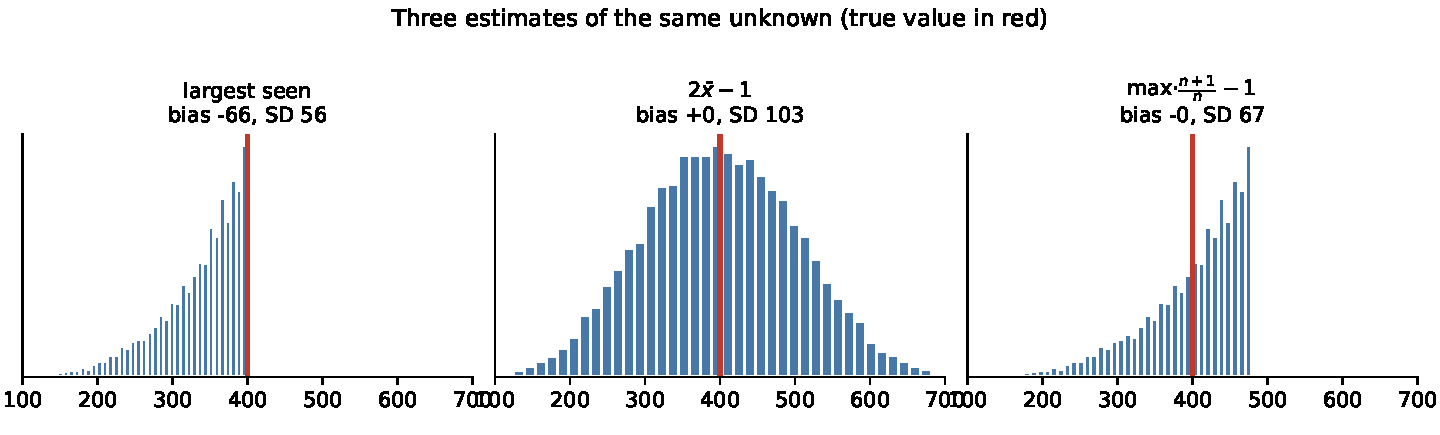
\includegraphics[width=0.95\textwidth]{fig_m08_tanks.pdf}
\end{center}
\vspace{-0.4em}
\small
With $N = 400$ and $n = 5$: the largest ticket seen is always too low (biased by $-66$). Doubling
the average is unbiased but wildly variable (SD 103). Correcting the maximum upward is both
unbiased and tight (SD 67), and it wins the contest.
\end{frame}

\begin{frame}{What this unit gives you}
\begin{columns}[T]
\begin{column}{0.5\textwidth}
\textbf{Things to know}
\begin{itemize}\small
  \item what an estimator is, and how to judge one by \textbf{bias}, \textbf{variance}, and MSE
  \item why the best estimator is often a slightly biased one
  \item shrinkage, and why every leaderboard needs it
  \item what a likelihood is, and what maximum likelihood actually maximizes
  \item why the curvature of the likelihood is the precision of the estimate
  \item how the bootstrap manufactures a sampling distribution from one sample
\end{itemize}
\end{column}
\begin{column}{0.5\textwidth}
\textbf{Mistakes to stop making}
\begin{itemize}\small
  \item chasing unbiasedness at the cost of enormous variance
  \item reporting an estimate with no standard error
  \item confusing the SD of the data with the SE of the estimate
  \item bootstrapping rows when the independent unit is a user, store, or week
  \item bootstrapping maxima or extreme quantiles
  \item ranking groups of very different sizes without shrinkage
\end{itemize}
\end{column}
\end{columns}
\end{frame}

% ======================================================================
\section{Judging estimators}
% ======================================================================
\begin{frame}{Three ways an estimate can be wrong}
\[
\underbrace{\E{(\hat\theta - \theta)^2}}_{\text{MSE}}
= \underbrace{(\E{\hat\theta} - \theta)^2}_{\text{bias}^2}
+ \underbrace{\mathrm{Var}(\hat\theta)}_{\text{variance}}
\]
\begin{itemize}
  \item \textbf{Bias:} on average, does it land on the truth?
  \item \textbf{Variance:} how much does it bounce from sample to sample?
  \item \textbf{MSE} combines them, and it is the number you should actually care about.
\end{itemize}
\begin{principle}{aim for accurate, not merely honest}
An estimator that is right on average but wildly variable is useless in the single sample you
actually have. You get one draw.
\end{principle}
\end{frame}

\begin{frame}{Why a biased estimator can win}
\begin{columns}[c]
\begin{column}{0.58\textwidth}
\centering
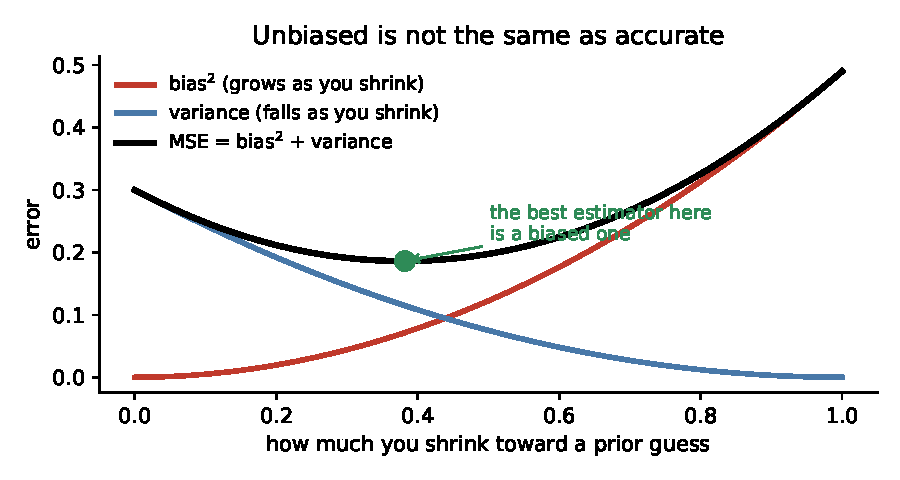
\includegraphics[width=\textwidth]{fig_m08_biasvar.pdf}
\end{column}
\begin{column}{0.42\textwidth}
\small
Pulling an estimate partway toward a sensible prior guess (\textbf{shrinkage}) buys a large drop
in variance for a small amount of bias.
\begin{itemize}
  \item Total error falls.
  \item This is the same tradeoff behind regularization, hierarchical models, and every
        ``smoothed'' metric you have seen.
\end{itemize}
\end{column}
\end{columns}
\end{frame}

\begin{frame}{The 3-for-3 salesperson}
\textbf{Setup.} A new rep closed all three of her first three deals. The unbiased estimate of her
close rate is 100\%.
\begin{itemize}
  \item Nobody believes 100\%. With three attempts, the estimate has enormous variance.
  \item A better estimate shrinks toward the company average: for instance, add the equivalent of
        a few ``average'' attempts before computing the rate.
  \item That is exactly how batting averages, restaurant ratings, and seller scores are computed
        in practice.
\end{itemize}
\begin{practice}{a favorite question}
``Which product has the best rating: 5.0 from 2 reviews, or 4.6 from 800?'' The answer requires
shrinkage, and saying so out loud is the point.
\end{practice}
\end{frame}

\begin{frame}{Your turn \#1}
\begin{yourturn}{design the leaderboard}
You run a marketplace. You must rank 10{,}000 sellers by customer rating. Some have 3 reviews,
some have 3{,}000.
\vspace{0.3em}

With a neighbor: what goes wrong if you rank by raw average? Propose a concrete fix, and say what
the fix costs you.
\end{yourturn}
\end{frame}

\begin{frame}{Your turn \#1: answer}
\begin{itemize}
  \item Raw averages put brand-new sellers with two five-star reviews at the top of every page.
        The leaderboard becomes a list of small samples, not good sellers.
  \item Fix: shrink each seller's average toward the site-wide average, with the weight depending
        on the review count. A seller with 3 reviews barely moves from the site average. A seller with
        3{,}000 keeps their own.
  \item The cost: genuinely excellent new sellers are understated for a while. That is the bias
        you are accepting in exchange for a stable, non-gameable ranking.
\end{itemize}
\begin{principle}{small samples must be handled, not trusted}
Any ranking built from unequal sample sizes needs shrinkage. Without it, you are ranking noise.
\end{principle}
\end{frame}

% ======================================================================
\section{Likelihood}
% ======================================================================
\begin{frame}{Where do estimators come from?}
Two general recipes:
\begin{itemize}
  \item \textbf{Method of moments:} choose the parameter that makes the model's mean match the
        sample mean. Simple, intuitive, occasionally poor.
  \item \textbf{Maximum likelihood:} choose the parameter under which the data you actually
        observed is most probable.
\end{itemize}
\begin{principle}{maximum likelihood in one sentence}
``Given this model, which parameter value would have made what I saw the least surprising?''
\end{principle}
\end{frame}

\begin{frame}{Method of moments, in one slide}
The simplest recipe there is: \emph{make the model's average match the data's average}, then solve.
\begin{itemize}
  \item Data: 40 support calls per day on average. Model: Poisson($\lambda$). Poisson's mean is
        $\lambda$, so set $\hat\lambda = 40$. Done.
  \item Data: mean 0.30 conversion. Model: Bernoulli($p$), whose mean is $p$, so $\hat p = 0.30$.
  \item It is quick, it is intuitive, and it often lands on the same answer as maximum likelihood.
\end{itemize}
\begin{trap}{where it falls apart}
Method of moments uses only the mean (and maybe the variance). It throws away the rest of the
data's shape, which is exactly the information you need when the model has several parameters or
the data is censored.
\end{trap}
\end{frame}

\begin{frame}{Likelihood, concretely}
You email 100 customers and 30 convert. If the true rate is $p$, the probability of seeing exactly
this data is
\[
L(p) = \binom{100}{30} p^{30} (1-p)^{70}.
\]
\begin{itemize}
  \item As a function of $p$, this is the \textbf{likelihood}. It is not a probability
        distribution over $p$. It ranks parameter values by how well they explain the
        data.
  \item It is maximized at $\hat p = 0.30$, the sample proportion. Maximum likelihood usually
        recovers the obvious estimator, and then keeps working when nothing is obvious.
\end{itemize}
\end{frame}

\begin{frame}{The curvature is the confidence}
\begin{columns}[c]
\begin{column}{0.58\textwidth}
\centering
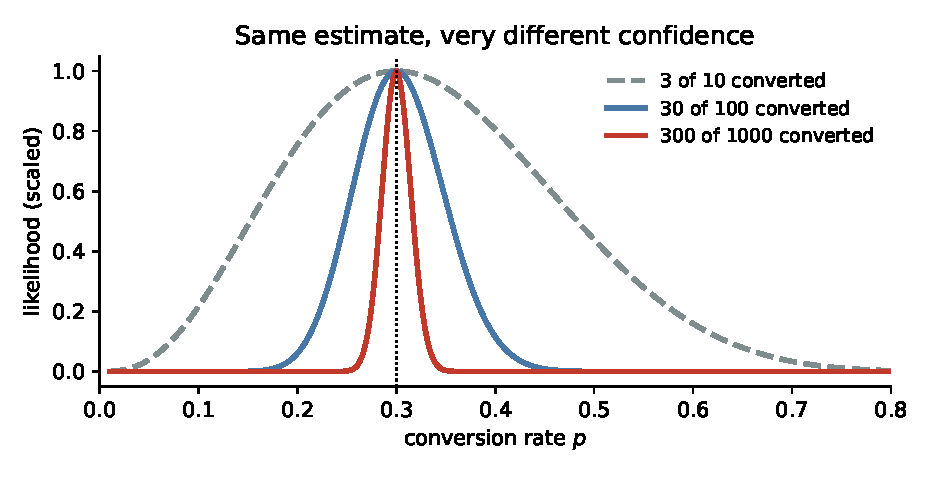
\includegraphics[width=\textwidth]{fig_m08_likelihood.pdf}
\end{column}
\begin{column}{0.42\textwidth}
\small
All three datasets estimate $\hat p = 0.30$. They are not equally convincing.
\begin{itemize}
  \item 3 of 10: a broad, flat curve. Many values explain the data nearly as well.
  \item 300 of 1000: a sharp spike. Only a narrow range is compatible.
\end{itemize}
\textbf{Sharp curve, small standard error.} That is where SEs come from in general.
\end{column}
\end{columns}
\end{frame}

\begin{frame}{Why this matters beyond the formula}
\begin{itemize}
  \item Every model you will fit later (logistic regression, Poisson regression, mixed models) is
        fit by maximizing a likelihood.
  \item Every standard error those models print comes from the curvature of that likelihood at
        its peak.
  \item So ``the model is very uncertain about this coefficient'' means ``the likelihood is flat
        in that direction,'' which usually means the data contains little information about it.
\end{itemize}
\begin{trap}{a flat likelihood still prints a number}
Software always prints a number. If two predictors are nearly identical, the likelihood is flat
along a ridge, and the individual coefficients are nearly arbitrary even though the fit is fine.
\end{trap}
\end{frame}

% ======================================================================
\section{The bootstrap}
% ======================================================================
\begin{frame}{The problem the bootstrap solves}
\begin{itemize}
  \item We know the standard error of a \emph{mean}: $\sigma/\sqrt{n}$.
  \item What is the standard error of a \textbf{median}? A 90th percentile? A ratio of two
        medians? The difference in churn between two segments after adjusting for tenure?
  \item Formulas exist for a few of these and nobody remembers them. The bootstrap needs none.
\end{itemize}
\begin{principle}{the bootstrap idea}
The sample is your best available picture of the population. So resample \emph{from the sample},
with replacement, and watch how much your estimate moves.
\end{principle}
\end{frame}

\begin{frame}{The bootstrap recipe}
\begin{enumerate}
  \item Draw a new sample of size $n$ from your data, \textbf{with replacement}.
  \item Compute your statistic on it. Anything at all: median, ratio, model coefficient.
  \item Repeat a few thousand times.
  \item The spread of those values is the standard error. The middle 95\% of them is a confidence
        interval.
\end{enumerate}
\vspace{0.3em}
\centering
Four lines of code, and it works for statistics that have no formula.
\end{frame}

\begin{frame}{The bootstrap, as code}
\begin{center}\small
\begin{minipage}{0.78\textwidth}
\texttt{boot = []}\\
\texttt{for i in range(5000):}\\
\texttt{\ \ \ \ resample = sample\_with\_replacement(data, size=len(data))}\\
\texttt{\ \ \ \ boot.append(your\_statistic(resample))}\\[4pt]
\texttt{se = std(boot)}\\
\texttt{ci = percentile(boot, [2.5, 97.5])}
\end{minipage}
\end{center}
\vspace{0.5em}
\begin{itemize}
  \item \texttt{your\_statistic} can be anything: a median, a 90th percentile, a ratio of two
        medians, an $R^2$, a model coefficient.
  \item Nothing in there assumes a distribution, requires a formula, or needs a derivation.
\end{itemize}
\end{frame}

\begin{frame}{Bootstrapping real data}
\begin{center}
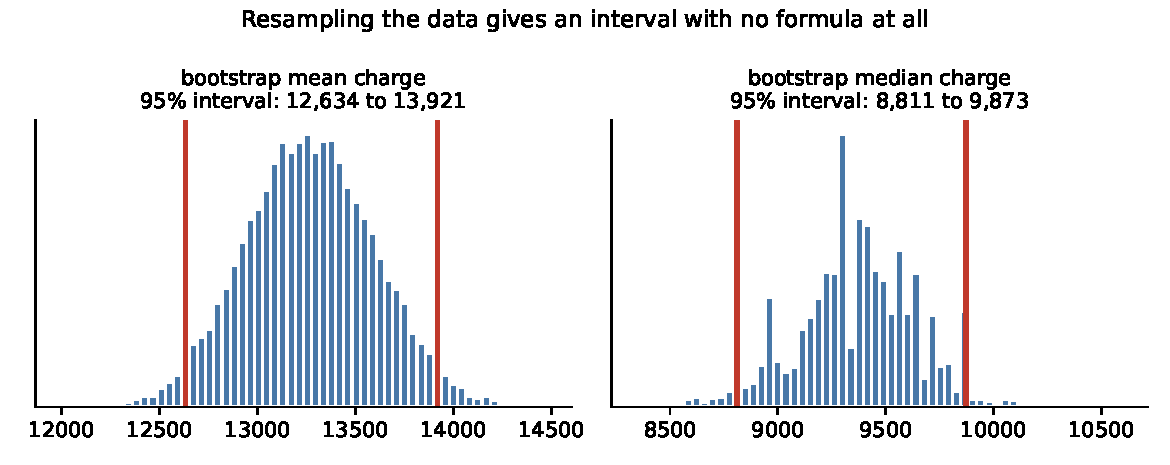
\includegraphics[width=0.95\textwidth]{fig_m08_bootstrap.pdf}
\end{center}
\vspace{-0.4em}
\small
Medical charges for 1{,}338 people. The mean and the median have very different intervals, and the
median's is far tighter, because it ignores the tail. Which one you report depends on the question,
not on which looks better.
\end{frame}

\begin{frame}{Your turn \#2}
\begin{yourturn}{which one do you report?}
Your company's charges data gives a bootstrap 95\% interval of roughly \$12{,}600 to \$13{,}900
for the \textbf{mean}, and \$8{,}800 to \$9{,}900 for the \textbf{median}.
\vspace{0.3em}

With a neighbor: give one business question where the mean is the right answer, and one where the
median is, and say why reporting only one could mislead.
\end{yourturn}
\end{frame}

\begin{frame}{Your turn \#2: answer}
\begin{itemize}
  \item \textbf{Mean:} anything about totals. Budgeting the year's payouts requires the mean,
        because the total is the mean times the number of people.
  \item \textbf{Median:} anything about a typical person. ``What does a customer like me pay?''
        is a median question.
  \item Reporting only the mean makes the typical experience sound worse than it is. Reporting
        only the median makes the budget look far too small.
\end{itemize}
\begin{principle}{the statistic follows the decision}
Choose the summary from what someone will \emph{do} with it, then bootstrap whatever you chose.
\end{principle}
\end{frame}

\begin{frame}{Three ways to get a standard error}
\begin{center}\small
\begin{tabular}{p{0.24\textwidth} p{0.34\textwidth} p{0.32\textwidth}}
\toprule
\textbf{Method} & \textbf{How} & \textbf{Use it when} \\
\midrule
Formula & $s/\sqrt{n}$ and its relatives & the statistic is a mean or a slope and the assumptions
hold \\
Likelihood curvature & how sharply the log-likelihood peaks & you fit a model by maximum
likelihood, which is what software reports \\
Bootstrap & resample and look at the spread & anything else, or when you do not trust the
formula's assumptions \\
\bottomrule
\end{tabular}
\end{center}
\vspace{0.4em}
\begin{principle}{they should agree, and it is worth checking}
On a well-behaved mean, all three land in the same place. When the bootstrap disagrees with the
formula, believe the bootstrap and go find out which assumption broke.
\end{principle}
\end{frame}

\begin{frame}{Where the bootstrap fails}
\begin{columns}[c]
\begin{column}{0.55\textwidth}
\centering
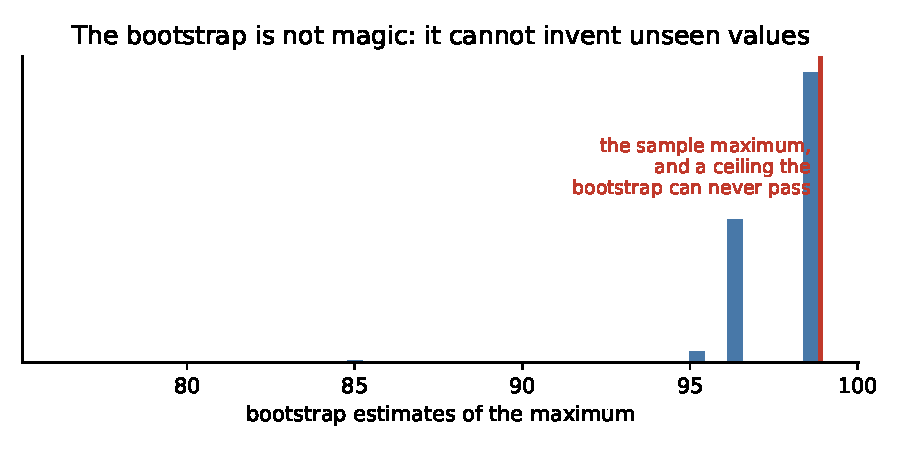
\includegraphics[width=\textwidth]{fig_m08_bootfail.pdf}
\end{column}
\begin{column}{0.45\textwidth}
\small
Resampling can never produce a value you did not observe, so it cannot see past the largest point
in your data.
\begin{itemize}
  \item Fails for maxima, minima, and extreme quantiles.
  \item Struggles with very small $n$, since it can only reshuffle what little you have.
  \item Breaks entirely on dependent data unless you resample \emph{clusters}.
\end{itemize}
\end{column}
\end{columns}
\end{frame}

\begin{frame}{Your turn \#3}
\begin{yourturn}{what is one observation?}
For each dataset, say what you would resample, and what your real $n$ is:
\begin{enumerate}
  \item Mean session length, from 100{,}000 page views by 6{,}000 visitors.
  \item Mean daily sales, from 365 consecutive days at one store.
  \item The district average, from 900 students in 30 classrooms.
\end{enumerate}
\end{yourturn}
\end{frame}

\begin{frame}{Your turn \#3: answer}
\begin{itemize}
  \item \textbf{Visitors}, not page views. Real $n$ is about 6{,}000, and resampling page views
        would understate the SE by roughly a factor of four.
  \item \textbf{Blocks of consecutive days}, not individual days. Sales are autocorrelated, so a
        day is not an independent draw, so resample contiguous stretches to keep the dependence.
  \item \textbf{Classrooms}, not students. Real $n$ is closer to 30 than 900, because students in
        a room share a teacher, a schedule, and a neighborhood.
\end{itemize}
\begin{principle}{the question that comes before the code}
``What is one independent observation?'' If you cannot answer it, no interval you compute means
anything, however sophisticated the method.
\end{principle}
\end{frame}

\begin{frame}{Bootstrapping dependent data, correctly}
\begin{itemize}
  \item If you have 100{,}000 sessions from 4{,}000 users, resampling \emph{sessions} pretends you
        have 100{,}000 independent pieces of information. Your interval will be far too narrow.
  \item Resample \textbf{users} instead, keeping all of a user's sessions together. Same idea for
        stores, classrooms, or hospitals.
  \item For time series, resample contiguous \emph{blocks} rather than individual days, to
        preserve the dependence.
\end{itemize}
\begin{trap}{the most common bootstrap error in industry}
Bootstrapping rows when the independent unit is something coarser. The code runs, the interval is
tight, and it is wrong.
\end{trap}
\end{frame}

% ======================================================================
\section{LLM check}
% ======================================================================
\begin{frame}{LLM check: mistake or not? (1 of 2)}
\begin{llmcheck}{we asked an LLM for an interval}
\textbf{We told it:} ``I have 500 session times and want a 95\% confidence interval for the
\emph{median} session time.''\\[4pt]
\textbf{It answered:} ``Compute the median, then use $\bar{x} \pm 1.96 \, s/\sqrt{n}$ with the
sample standard deviation. That gives a 95\% confidence interval for the median.''
\end{llmcheck}
\vspace{0.2em}
\centering\small Mistake, or no mistake?
\onslide<2->{%
\begin{trap}{verdict: mistake}
That formula is the interval for the \emph{mean}, and on skewed session times the mean and median
are far apart. The clean answer is to bootstrap the median directly, which needs no formula at
all.
\end{trap}}
\end{frame}

\begin{frame}{LLM check: mistake or not? (2 of 2)}
\begin{llmcheck}{same territory, a different answer}
\textbf{We told it:} ``We have 80{,}000 support tickets from 5{,}000 customers. Bootstrap the
average resolution time.''\\[4pt]
\textbf{It answered:} ``I would resample \emph{customers}, not tickets, keeping each customer's
tickets together. Tickets from the same customer are correlated, so resampling tickets would treat
80{,}000 rows as independent and produce an interval that is much too narrow.''
\end{llmcheck}
\vspace{0.2em}
\centering\small Mistake, or no mistake?
\onslide<2->{%
\begin{principle}{verdict: no mistake}
It identified the independent unit before writing any code. That single habit separates a
defensible interval from a confident-looking one.
\end{principle}}
\end{frame}

% ======================================================================
\section{Workflow}
% ======================================================================
\begin{frame}{How to estimate anything, in order}
\begin{enumerate}
  \item \textbf{Write the target in words.} ``Median revenue per active user in Q3,'' not
        ``revenue.''
  \item \textbf{Identify the independent unit.} Users? Stores? Weeks? This decides your real $n$.
  \item \textbf{Choose the statistic from the decision}, not from convenience.
  \item \textbf{Compute the estimate}, then immediately ask how much it would move on a fresh
        sample.
  \item \textbf{Get the uncertainty}: a formula if one applies, otherwise a bootstrap over the
        independent unit.
  \item \textbf{Consider shrinkage} if any group has a small sample.
  \item \textbf{Report estimate, interval, and the assumption you are least sure about.}
\end{enumerate}
\end{frame}

\begin{frame}{Scenario: the regional conversion leaderboard}
\textbf{Setup.} Marketing ranks 40 regions by conversion rate. The top region converts at 22\% against a
company average of 9\%. They want to copy that region's playbook everywhere.
\begin{itemize}
  \item First question: how many visitors did that region have? If the answer is 45, its 22\% is
        one lucky week.
  \item Second: with 40 regions, the maximum of 40 noisy estimates is high \emph{by construction},
        even if all regions are identical.
  \item What to do: shrink each region's rate toward the company average, bootstrap the intervals,
        and check whether next quarter's data agrees.
\end{itemize}
\begin{interview}{how to answer}
``The winner of a leaderboard is a biased estimate of the best performer. I would shrink, then
validate on new data before rolling out a playbook.''
\end{interview}
\end{frame}

% ======================================================================
\section{Consolidate}
% ======================================================================
\begin{frame}{Estimating anything, with an interval}
\small
\begin{enumerate}
  \item \textbf{Write the target in words and units}, for example ``median revenue per active user.''
  \item \textbf{Identify the independent unit}: users, stores, or weeks. This sets your real $n$.
  \item \textbf{Choose the statistic from the decision}, not from convenience.
  \item \textbf{Compute the estimate.}
  \item \textbf{Resample with replacement} a few thousand times, recomputing the statistic each time.
  \item \textbf{Take the SD of those values} for the standard error and the 2.5 and 97.5 percentiles for the interval.
  \item \textbf{Shrink toward a sensible prior} if any group has a small sample, then report estimate, interval, and the shakiest assumption.
\end{enumerate}
\end{frame}

\begin{frame}{The traps, all in one place}
\begin{trap}{the ones that bite most often}
\begin{itemize}
  \item Treating unbiasedness as the only virtue and ignoring variance.
  \item Reporting a point estimate with no standard error or interval.
  \item Confusing the SD of the data with the SE of the estimate.
  \item Bootstrapping rows when the independent unit is a user, store, or week.
  \item Bootstrapping maxima or extreme quantiles.
  \item Ranking groups of very different sizes without shrinkage.
\end{itemize}
\end{trap}
\end{frame}

\begin{frame}{Ten questions to be able to answer}
\begin{enumerate}\small
  \item What makes one estimator better than another? Define bias, variance, and MSE.
  \item Give an example where a biased estimator is the better choice.
  \item Explain maximum likelihood in plain English.
  \item Why does the shape of the likelihood tell you the standard error?
  \item How would you get a confidence interval for a 90th percentile?
  \item Explain the bootstrap to a product manager in thirty seconds.
  \item When does the bootstrap fail, and what would you do instead?
  \item We have 80{,}000 rows from 5{,}000 customers. What do you resample?
  \item A new rep is 3-for-3. What is your estimate of her close rate?
  \item How would you build a leaderboard that new sellers cannot game with two reviews?
\end{enumerate}
\end{frame}

\begin{frame}{Mastery checklist}
You have this unit when you can, from memory:
\begin{itemize}
  \item decompose an estimator's error into bias and variance and argue about the tradeoff
  \item explain why shrinkage improves small-sample estimates
  \item define the likelihood and say what maximum likelihood chooses
  \item connect the curvature of the likelihood to the standard error
  \item run and explain a bootstrap, including the choice of resampling unit
  \item name three situations where the bootstrap should not be trusted
\end{itemize}
\end{frame}

\begin{frame}{What you should be able to do with software}
\small
Nobody is asking you to memorize syntax. You are expected to know \emph{which} procedure the
question calls for, what to hand it, and what the output means. With an AI assistant open, you
should be able to produce any of these and defend the result.
\begin{center}\footnotesize
\begin{tabular}{p{0.44\textwidth} p{0.46\textwidth}}
\toprule
\textbf{You should be able to} & \textbf{What you would reach for} \\
\midrule
Resample rows with replacement & \texttt{rng.integers(0, n, size=(B, n))} \\
Bootstrap SE and percentile interval & \texttt{boot.std()}, \texttt{np.percentile(boot, [2.5, 97.5])} \\
Bootstrap a median, a percentile, or a ratio & the same loop, a different statistic \\
Resample clusters instead of rows & sample the group labels, then pool their rows \\
Maximum likelihood for a simple model & \texttt{scipy.optimize.minimize} on the negative log-likelihood \\
Bias, variance, and MSE of an estimator & simulate from a known truth and compare \\
Shrunken group estimates & \texttt{(sum + k*overall) / (n + k)} \\
\bottomrule
\end{tabular}
\end{center}
\vspace{0.2em}
\centering\small
If you cannot say what the output means, the fact that you produced it is worth nothing.
\end{frame}

\begin{frame}{Where we go next}
\begin{itemize}
  \item You can now produce an estimate and an honest interval for almost any quantity, with or
        without a formula. That closes out the foundations.
  \item \textbf{Unit 2} puts the machinery to work on a relationship rather than a single number:
        regression, where the estimate is a slope and every idea from Units 1 through 4 comes back
        wearing new clothes.
\end{itemize}
\begin{principle}{the through-line}
Estimation is not about getting a number. It is about knowing how much that number would have
changed if the world had rolled the dice again.
\end{principle}
\end{frame}

\end{document}
